\documentclass[12pt,a4paper]{article}
\usepackage[left=30mm,right=15mm,top=20mm,bottom=20mm]{geometry}
\usepackage{fontspec}
\usepackage{polyglossia}
\setmainlanguage{russian}
\setotherlanguage{english}
\setmainfont[Ligatures=TeX]{PT Serif}
\setsansfont[Ligatures=TeX]{PT Sans}
\setmonofont[Scale=0.85]{PT Mono}
\newfontfamily\cyrillicfont[Ligatures=TeX,Script=Cyrillic]{PT Serif}
\newfontfamily\cyrillicfontsf[Ligatures=TeX,Script=Cyrillic]{PT Sans}
\newfontfamily\cyrillicfonttt[Scale=0.85,Script=Cyrillic]{PT Mono}
\usepackage{xcolor}
\definecolor{accent}{HTML}{1F4E79}
\definecolor{boxbg}{HTML}{EAF1F8}
\usepackage{graphicx}
\usepackage{booktabs}
\usepackage{array}
\usepackage{caption}
\usepackage{amsmath}
\usepackage{enumitem}
\usepackage{setspace}
\usepackage{titlesec}
\usepackage{tcolorbox}
\usepackage{fancyvrb}
\setstretch{1.15}
\setlength{\parindent}{1.25cm}
\setlist{nosep,leftmargin=1.5em}
\titleformat{\section}{\large\bfseries\color{accent}}{\thesection}{0.6em}{}
\titleformat{\subsection}{\normalsize\bfseries}{\thesubsection}{0.6em}{}
\DeclareCaptionLabelSeparator{gost}{~--- }
\captionsetup[table]{font=small,labelfont=bf,labelsep=gost,skip=4pt,justification=raggedright,singlelinecheck=false}
\captionsetup[figure]{font=small,labelfont=bf,labelsep=gost,skip=4pt}
\usepackage[hidelinks]{hyperref}
\usepackage[normalem]{ulem}
\let\plainhref\href
\renewcommand{\href}[2]{\plainhref{#1}{\uline{\textcolor{accent}{#2}}}}
\newcommand{\tabcap}[1]{\captionof{table}{#1}}
\newenvironment{gosttable}[1]{\begin{center}\begin{minipage}{\linewidth}\tabcap{#1}\centering\small}{\end{minipage}\end{center}}
\setcounter{tocdepth}{2}
\makeatletter\let\inputtab\@@input\makeatother
\setlength{\emergencystretch}{3em}
\usepackage{float}


\begin{document}

\begin{titlepage}
\centering
{\large Санкт-Петербургский государственный университет\par}
\vspace{3cm}
{\large Проект по дисциплине <<Статистические методы>>\par}
\vspace{3cm}
{\LARGE\bfseries Статистический анализ качества RAG\par}
\vspace{0.8cm}
{\large Влияние параметров поиска и свойств вопроса на качество ответа: HotpotQA и SQuAD\par}
\vspace{4cm}
\begin{flushright}
Выполнил: Ручьев И.\,А.\par
\end{flushright}
\vfill
{Санкт-Петербург, 2026\par}
\end{titlepage}

\begin{tcolorbox}[colback=boxbg,colframe=accent,boxrule=0.6pt,arc=0pt,left=8pt,right=8pt,top=6pt,bottom=6pt]
\small
Система RAG (BM25, плотный и гибридный поиск + экстрактивный ридер) прогнана на 600 вопросах HotpotQA и 600 вопросах SQuAD по сетке из 72 конфигураций: ретривер, top-k, размер чанка. Отдельно прогнан итеративный поиск в 4 шага. По логам поиска и ответов проверены шесть гипотез, построены регрессия F1 и классификатор правильности.

Параметры системы значимо меняют полноту поиска, но внутри датасета объясняют около 1\,\% дисперсии F1 ответа; на вопрос приходится 60--68\,\%. Прирост F1 от top-5 к top-10 не превышает 0,018. Итеративный поиск повышает полноту на многошаговых вопросах на 4,5 пункта, на одношаговых снижает ее; на F1 итерации сами по себе не влияют. Правильность предсказуема по логу без эталона с ROC-AUC 0,84.
\end{tcolorbox}

\tableofcontents
\newpage

\section{Введение}

\textbf{Актуальность.} Генерация с дополненным поиском (Retrieval-Augmented Generation, RAG\footnote{RAG --- схема, в которой ответ модели строится по фрагментам документов, найденным поиском по запросу пользователя~\cite{lewis2020}.}) стала стандартной архитектурой вопросно-ответных систем над корпоративными и открытыми базами знаний. Качество такой системы зависит от набора параметров: способа поиска, числа фрагментов, передаваемых модели (top-k), размера фрагмента (чанка) и числа шагов поиска. На практике эти параметры подбирают по средним значениям метрик на небольших наборах вопросов, без проверки того, что разница между конфигурациями не случайна. Сравнения систем поиска без статистических тестов --- известная проблема в информационном поиске и NLP~\cite{smucker2007,dror2018}.

\textbf{Цель} --- статистически оценить, какие параметры RAG и какие свойства вопроса значимо влияют на качество поиска и ответа, и насколько правильность ответа предсказуема по логам.

\textbf{Задачи:}
\begin{enumerate}
\item выбрать и обосновать датасеты из пяти заданных (MS MARCO, Natural Questions, HotpotQA, BEIR, SQuAD);
\item прогнать систему ретривер\,+\,ридер по сетке параметров и записать логи поиска и ответов;
\item получить описательную статистику метрик по конфигурациям;
\item проверить гипотезы о влиянии параметров и свойств вопроса на качество;
\item оценить корреляции параметров и метрик;
\item построить регрессию качества по параметрам и классификатор правильности ответа;
\item оценить динамику качества по итерациям поиска.
\end{enumerate}

\textbf{Гипотезы.}
\begin{itemize}
\item[H1.] Тип ретривера (BM25, плотный, гибридный) значимо влияет на полноту поиска и на F1 ответа.
\item[H2.] С ростом top-k полнота поиска монотонно растет, а F1 ответа растет медленнее и выходит на плато.
\item[H3.] Размер чанка значимо влияет на качество ответа.
\item[H4.] На многошаговых вопросах качество ниже на вопросах типа bridge, чем comparison, и падает с ростом уровня сложности.
\item[H5.] Наличие ответа в найденном контексте повышает шанс правильного ответа, но не гарантирует его.
\item[H6.] Итеративный поиск повышает полноту на многошаговых вопросах по сравнению с одношаговым поиском того же объема контекста и не дает выигрыша на одношаговых.
\end{itemize}

\section{Обзор датасетов}

Преподавателем заданы пять наборов данных; дополнительно рассмотрены три близких набора для многошаговых и открытых вопросов. Характеристики --- в таблице~\ref{tab:datasets}. BEIR включает в себя Natural Questions, HotpotQA и MS MARCO как подзадачи поиска, но без ответов, поэтому он рассматривается как источник разметки релевантности, а не как отдельный корпус.

\begin{gosttable}{Рассмотренные датасеты: пять заданных и три дополнительных}\label{tab:datasets}
\begin{tabular}{>{\raggedright\arraybackslash}p{2.5cm}>{\raggedright\arraybackslash}p{3.4cm}>{\raggedright\arraybackslash}p{4.1cm}>{\raggedright\arraybackslash}p{4.1cm}}
\toprule
Датасет & Объем & Что размечено & Ограничение для задачи \\
\midrule
MS MARCO~\cite{msmarco} & 1\,010\,916 запросов Bing, 8,8~млн пассажей & 10 пассажей выдачи Bing на запрос с отметкой полезности, свободный ответ человека & ответы перефразированы, F1 к ним занижен у экстрактивного ридера; корпус тяжелый \\
Natural Questions~\cite{nq} & 307\,373 обучающих вопроса, 7\,830 dev & реальные запросы Google, длинный и короткий ответ на странице Википедии & корпус --- полные страницы, архив около 40~ГБ \\
HotpotQA~\cite{hotpotqa} & 90\,447 train, 7\,405 dev (distractor) & 2 нужных абзаца и 8 отвлекающих, опорные предложения, тип bridge/comparison, уровень easy/medium/hard & в dev все вопросы уровня hard \\
BEIR~\cite{beir} & 18 наборов, 9 типов задач & запросы и релевантность документов & нет ответов --- только поиск \\
SQuAD v1.1~\cite{squad} & 87\,599 train, 10\,570 dev, 536 статей & ответ --- отрезок абзаца Википедии & вопросы написаны по абзацу, высокое лексическое пересечение \\
\midrule
2Wiki\-Multihop\-QA~\cite{twowiki} & 192\,606 вопросов & 2--4 нужных абзаца, цепочка фактов из Викиданных & вопросы шаблонные, вне заданного списка \\
MuSiQue~\cite{musique} & около 25 тыс. вопросов на 2--4 шага & нужные абзацы, разбиение на подвопросы & вне заданного списка, вопросы собраны из одношаговых \\
TriviaQA~\cite{triviaqa} & 95 тыс. пар вопрос--ответ, 650 тыс. документов & ответ и найденные документы без разметки нужного абзаца & нет разметки релевантности --- не измерить поиск \\
\bottomrule
\end{tabular}
\end{gosttable}

Для анализа выбраны \textbf{HotpotQA} и \textbf{SQuAD v1.1} из заданного списка.
\begin{itemize}
\item В обоих есть и разметка релевантности (нужные абзацы и опорные предложения у HotpotQA, исходный абзац у SQuAD), и эталонный ответ. Это позволяет отдельно мерить поиск и ответ в одном логе.
\item Ответы в обоих экстрактивные --- это отрезок текста, поэтому EM и F1 корректны без LLM-судьи.
\item HotpotQA дает факторы вопроса для гипотез: тип (bridge --- ответ через промежуточную сущность, comparison --- сравнение двух объектов) и уровень сложности.
\item SQuAD --- одношаговые вопросы. Он служит контрольной группой для итеративного поиска и для эффекта лексического пересечения.
\item Оба набора умещаются в память ноутбука: прогон воспроизводим без GPU-сервера.
\end{itemize}

MS MARCO и Natural Questions не выбраны из-за объема корпуса и свободной формы ответов. BEIR не содержит ответов, поэтому на нем не измерить вторую половину RAG.

\section{Обзор методов}

\textbf{Схема ретривер--ридер.} Chen и соавторы~\cite{drqa} предложили для открытых вопросов по Википедии двухступенчатую схему: TF-IDF-поиск абзацев и нейросетевой ридер, выделяющий ответ. Lewis и соавторы~\cite{lewis2020} заменили ридер генератором и ввели название RAG. Обзор~\cite{gao2023} выделяет параметры, которые подбирают на практике: тип ретривера, размер чанка, top-k, итеративный поиск. Эта работа использует ту же схему с экстрактивным ридером.

\textbf{Ретриверы.} BM25~\cite{bm25} --- лексическая модель ранжирования, базовая линия во всех бенчмарках поиска. Плотный поиск DPR~\cite{dpr} на Natural Questions превзошел BM25 по точности top-20 на 9--19 процентных пунктов. Эмбеддинги E5~\cite{e5} обучены контрастивно на слабой разметке и сильны без дообучения. Слияние выдач через RRF~\cite{rrf}\footnote{Reciprocal Rank Fusion: документ получает сумму $1/(60+r_i)$ по рангам $r_i$ в каждой выдаче.} устойчиво превосходит отдельные системы. BEIR~\cite{beir} показал, что вне домена обучения BM25 часто сильнее плотных моделей. Поэтому тип ретривера --- фактор с неочевидным знаком эффекта.

\textbf{Оценка RAG.} RAGAS~\cite{ragas} и ARES~\cite{ares} оценивают верность ответа контексту и релевантность контекста LLM-судьей, ARES --- с доверительными интервалами по малой размеченной выборке. eRAG~\cite{erag} показал, что классические метрики поиска по разметке релевантности слабо коррелируют с итоговым качеством RAG, и предложил оценивать документ по тому, помогает ли он ответить. Здесь та же связь проверяется прямой корреляцией полноты поиска и F1 ответа.

\textbf{Влияние контекста.} Liu и соавторы~\cite{lostmiddle} показали, что качество ответа падает, когда нужный фрагмент в середине длинного контекста, и что рост числа документов перестает помогать. Cuconasu и соавторы~\cite{powernoise} измерили влияние отвлекающих документов на точность RAG на Natural Questions. Это основа гипотезы H2 о плато.

\textbf{Итеративный поиск.} IRCoT~\cite{ircot} чередует шаги поиска и рассуждения и на четырех многошаговых наборах, включая HotpotQA, повышает полноту поиска до 21 пункта против одношагового поиска. В этой работе используется упрощенный вариант без LLM: к запросу дописывается промежуточный ответ ридера.

\textbf{Статистическое сравнение систем.} Smucker и соавторы~\cite{smucker2007} сравнили тесты значимости для оценки поиска и рекомендовали парные тесты на одних и тех же запросах. Dror и соавторы~\cite{dror2018} дали схему выбора теста для метрик NLP: для ненормальных и ограниченных метрик --- непараметрические парные тесты, при множественных сравнениях --- поправка. Отсюда методика этой работы: тест Фридмана~\cite{friedman} и Вилкоксона для F1 и полноты, Q Кохрена~\cite{cochran} и Мак-Немара~\cite{mcnemar} для бинарной правильности, тренд Пейджа~\cite{page} для упорядоченных уровней, поправка Холма~\cite{holm}, бутстреп-интервалы~\cite{efron}. Наблюдения одного вопроса в разных конфигурациях зависимы, поэтому регрессия считается с кластерными ошибками, а логистическая --- методом обобщенных оценочных уравнений (GEE~\cite{gee}).

\section{Методология и пайплайн анализа}

\subsection{Данные и выборка}

Из HotpotQA (distractor, train: 17\,972 вопроса easy, 56\,814 medium, 15\,661 hard) взято по 200 вопросов каждого уровня без ответов yes/no\footnote{Ответы yes/no не встречаются в тексте как отрезок, экстрактивный ридер их не выдает; таких вопросов в train 6\,\%.}. Корпус --- все абзацы выбранных вопросов: два нужных и восемь отвлекающих на вопрос, после удаления повторов по заголовку. Отвлекающие абзацы в HotpotQA подобраны поиском по биграммам, то есть корпус заведомо содержит лексически похожие документы. Из SQuAD v1.1 dev взято 600 случайных вопросов, корпус --- все 2\,067 абзацев dev-части. Зерно выборки --- 42.

\subsection{Система RAG и сетка параметров}

\begin{itemize}
\item \textbf{Чанки:} документы режутся по предложениям до 50, 100 или 200 слов, к чанку приписывается заголовок документа.
\item \textbf{Ретриверы:} BM25 (bm25s, $k_1=1{,}5$, $b=0{,}75$), плотный intfloat/e5-small-v2, гибрид через RRF по выдачам глубины 50.
\item \textbf{top-k:} 1, 3, 5, 10.
\item \textbf{Ридер:} deepset/roberta-base-squad2. На каждый чанк выдачи ищется лучший отрезок, ответ системы --- отрезок с наибольшей оценкой среди top-k чанков.
\end{itemize}

Сетка: 2 датасета $\times$ 3 ретривера $\times$ 3 размера чанка $\times$ 4 значения top-k = 72 конфигурации, по 600 вопросов в каждой --- 43\,200 строк лога ответов. Лог поиска хранит выдачу глубины 10 с оценкой ретривера, отметкой релевантности и ответом ридера на каждый чанк.

\textbf{Итеративный поиск} (гибрид, чанк 100): на шаге $t$ в контекст добавляются 3 новых чанка, к запросу дописывается ответ ридера по новым чанкам. Контроль --- одношаговый поиск того же объема (top-$3t$). Шагов 4.

\subsection{Метрики}

\begin{itemize}
\item \textbf{Релевантный чанк}: у HotpotQA --- чанк нужного абзаца, содержащий опорное предложение; у SQuAD --- чанк исходного абзаца, содержащий ответ (если ответ разрезан границей чанков --- все чанки абзаца).
\item \textbf{Полнота поиска} (recall@k) --- доля нужных документов вопроса, релевантный чанк которых попал в top-k (у HotpotQA нужных два, у SQuAD один).
\item \textbf{Попадание} (hit@k) --- в top-k есть хотя бы один релевантный чанк. \textbf{MRR@k} --- обратный ранг первого релевантного чанка.
\item \textbf{Ответ в контексте} --- эталонный ответ встречается подстрокой в top-k чанках.
\item \textbf{EM} --- точное совпадение после нормализации SQuAD. \textbf{F1} --- гармоническое среднее точности и полноты по словам ответа~\cite{squad}.
\item \textbf{Правильный ответ} --- F1~$\ge 0{,}5$.
\item \textbf{Лексическое пересечение} --- доля значимых слов вопроса (без стоп-слов), встречающихся в эталонных абзацах; считается по эталону и описывает вопрос, а не систему.
\end{itemize}

\subsection{Пайплайн анализа}

\begin{enumerate}
\item Описательная статистика по конфигурациям, бутстреп-интервалы (2\,000 повторов).
\item Парные тесты по вопросам: Фридман, Вилкоксон (нулевые разности отбрасываются) для F1, Q Кохрена и Мак-Немар для бинарных метрик, тренд Пейджа, поправка Холма, бутстреп-интервал парной разности и TOST для проверки плато. Межгрупповые: Манн--Уитни, Краскел--Уоллис, $\chi^2$.
\item Корреляции Спирмена по всей сетке, проверка значимости ключевых пар.
\item OLS для F1 с кластерными ошибками по вопросу, GEE-логит для правильности, VIF и остатки.
\item Классификация правильности по признакам без эталона: логистическая регрессия и градиентный бустинг, 5-кратная групповая кросс-валидация по вопросу.
\item Динамика по итерациям: Фридман и тренд Пейджа, Вилкоксон итеративный против одношагового, GEE с взаимодействием итерация $\times$ режим.
\end{enumerate}

Структура логов --- в приложении~\ref{app:logs}, команды воспроизведения --- в приложении~\ref{app:repro}.

\section{Результаты}

\subsection{Описательная статистика}

Выборка HotpotQA --- 600 вопросов: по 200 уровней easy, medium, hard; 504 вопроса типа bridge и 96 типа comparison. Корпус HotpotQA --- 5\,904 абзаца, SQuAD --- 2\,067 абзацев. Число чанков приведено в таблице~\ref{tab:corpus}.

\begin{gosttable}{Корпуса и вопросы}\label{tab:corpus}
\begin{tabular}{lrrrrrr}
\toprule
Датасет & Абзацев & \multicolumn{3}{c}{Чанков при размере, слов} & Длина вопроса, & Пересечение \\
 & & 50 & 100 & 200 & слов (медиана) & с эталоном\footnotemark \\
\midrule
HotpotQA & 5\,904 & 14\,659 & 8\,136 & 6\,097 & 17 & 0,823 \\
SQuAD & 2\,067 & 6\,859 & 3\,630 & 2\,222 & 10 & 0,670 \\
\bottomrule
\end{tabular}
\end{gosttable}
\footnotetext{Доля значимых слов вопроса (без стоп-слов), встречающихся в эталонных абзацах; среднее по вопросам.}

Таблица~\ref{tab:desc} --- метрики базовой конфигурации: чанк 100 слов, top-5. В квадратных скобках --- 95\,\% бутстреп-интервал (2\,000 повторов).

\begin{gosttable}{Качество поиска и ответа в базовой конфигурации (чанк 100, top-5)}\label{tab:desc}
\begin{tabular}{llccc}
\toprule
Датасет & Ретривер & Полнота поиска & F1 ответа & Доля правильных \\
\midrule
\inputtab tables/tab_desc.tex 
\bottomrule
\end{tabular}
\end{gosttable}

Стандартное отклонение F1 --- от 0,46 на HotpotQA до 0,36--0,38 на SQuAD, медиана F1 на SQuAD равна 1 у всех ретриверов. Распределение F1 бимодально (рисунок~\ref{fig:dist}): у HotpotQA (гибрид) 42,3\,\% ответов имеют F1~=~0 и 41,2\,\% --- F1~=~1, у SQuAD --- 14,0\,\% и 75,7\,\%. Тест Шапиро--Уилка по всем 600 вопросам отвергает нормальность с $p < 10^{-29}$ в обоих наборах. Поэтому для F1 дальше используются ранговые тесты, а для бинарной правильности --- тесты для долей.

\begin{figure}[ht]
\centering
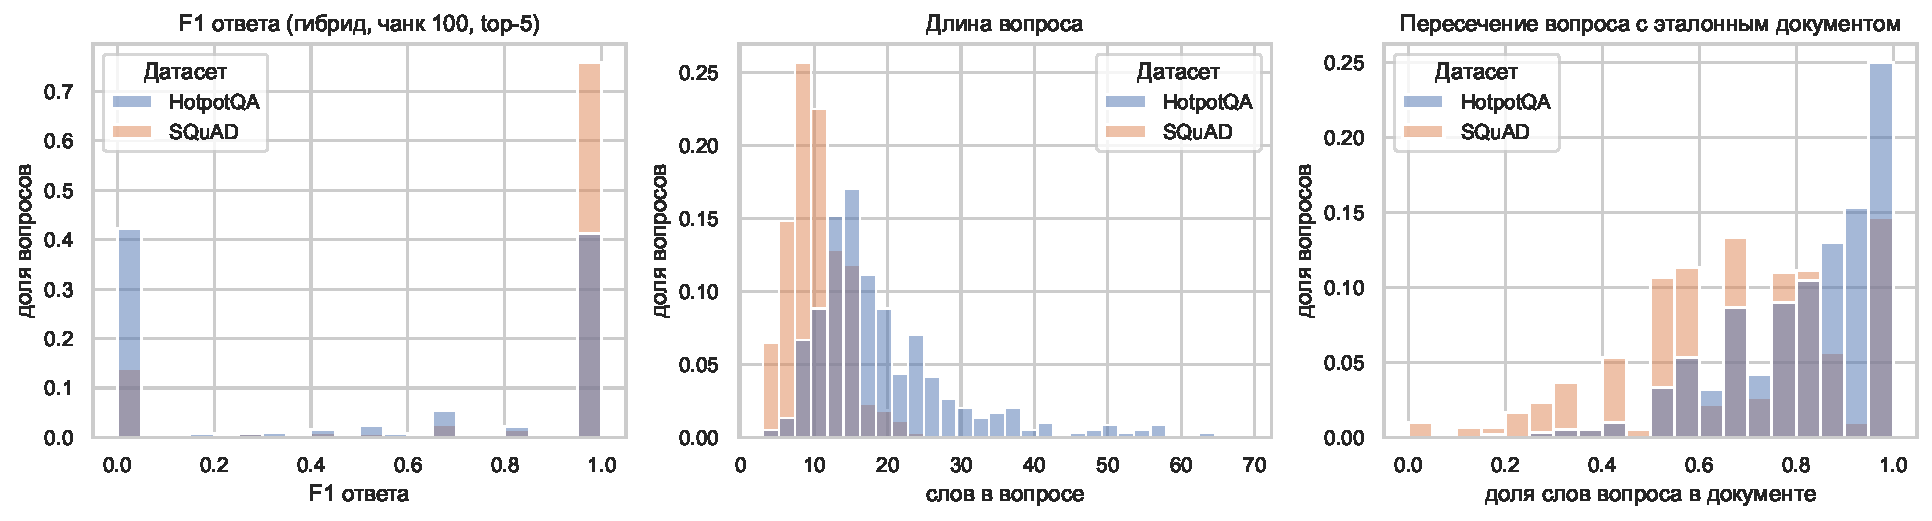
\includegraphics[width=\linewidth]{figures/distributions.pdf}
\caption{Распределения F1 ответа, длины вопроса и лексического пересечения}\label{fig:dist}
\end{figure}

HotpotQA сложнее SQuAD по всем метрикам: при гибридном поиске F1 0,503 против 0,817. При этом ответ присутствует в найденном контексте у 79,7\,\% вопросов HotpotQA и 96,2\,\% вопросов SQuAD. Полные таблицы по 72 конфигурациям --- в приложении~\ref{app:grid}.

\subsection{Проверка гипотез}

Сводка --- в таблице~\ref{tab:hyp}. Для парных сравнений (один вопрос во всех конфигурациях) база --- чанк 100 и top-5, для H2 и H3 ретривер фиксирован --- гибрид. Уровень значимости 0,05, попарные сравнения с поправкой Холма. Для F1 и полноты HotpotQA (значения 0; 0,5; 1) --- знаково-ранговый тест Вилкоксона с отбрасыванием нулевых разностей, для бинарных метрик (полнота SQuAD, попадание, правильность) --- тест Мак-Немара. Для каждой пары приведена средняя парная разность и ее бутстреп-интервал.

\begin{gosttable}{Результаты проверки гипотез}\label{tab:hyp}
\begin{tabular}{>{\raggedright\arraybackslash}p{0.7cm}>{\raggedright\arraybackslash}p{2.8cm}>{\raggedright\arraybackslash}p{4.5cm}>{\raggedright\arraybackslash}p{3.5cm}>{\raggedright\arraybackslash}p{2.8cm}}
\toprule
№ & Тест & HotpotQA & SQuAD & Вывод \\
\midrule
H1 & Фридман, Q Кохрена & полнота: $\chi^2 = 170{,}9$, $p < 10^{-37}$, $W = 0{,}14$; F1: $\chi^2 = 31{,}7$, $p = 1{,}3 \cdot 10^{-7}$, $W = 0{,}03$ & полнота: $p = 4{,}5 \cdot 10^{-5}$; F1: $p = 0{,}049$, гибрид лучше BM25 на 0,026 & подтверждена; на SQuAD эффект на ответ мал \\
H2 & тренд Пейджа, парная разность $k{=}10$ и $k{=}5$ & полнота: $+0{,}084$, $p < 10^{-21}$; F1: $-0{,}003$ [$-0{,}024$; $0{,}018$] & полнота: $+0{,}028$, $p = 10^{-4}$; F1: $-0{,}010$ [$-0{,}024$; $0{,}004$] & рост F1 после $k{=}5$ не выше 0,018 \\
H3 & Фридман, Q Кохрена & F1: $p = 0{,}66$; полнота: $p = 3{,}4 \cdot 10^{-11}$ & F1: $p = 0{,}23$; полнота: $p = 8{,}6 \cdot 10^{-5}$ & для F1 не подтверждена \\
H4 & Манн--Уитни, Краскел--Уоллис, $\chi^2$ & comparison хуже bridge, $p = 0{,}004$; easy лучше medium и hard, $p_{Holm} = 1{,}3 \cdot 10^{-6}$ & --- & частично \\
H5 & точный тест Фишера & отношение шансов 55, $p < 10^{-39}$ & отношение шансов 40, $p < 10^{-13}$ & подтверждена \\
H6 & Вилкоксон, Мак-Немар, Фридман, GEE & полнота на шаге 2: 0,916 против 0,871, $p_{Holm} = 1{,}7 \cdot 10^{-8}$; F1 не меняется & полнота на шаге 4 ниже: 0,970 против 0,987, $p_{Holm} = 0{,}028$; F1 как у одношагового & подтверждена для поиска; на SQuAD итерации снижают полноту \\
\bottomrule
\end{tabular}
\end{gosttable}

\textbf{H1, ретривер.} На HotpotQA плотный поиск превосходит BM25 по полноте на 12,8 пункта (0,866 против 0,738, интервал разности [0,107; 0,152], Вилкоксон $p_{Holm} = 2{,}7 \cdot 10^{-24}$) и по F1 на 5,8 пункта ([0,035; 0,082], $p_{Holm} = 8{,}5 \cdot 10^{-6}$). Плотный поиск находит больше гибрида (разность полноты 0,026, $p = 0{,}001$), но по F1 они не различаются ($p = 0{,}21$). На SQuAD тип ретривера меняет полноту: гибрид 0,953 против 0,905 у BM25 (Мак-Немар $p_{Holm} = 5{,}9 \cdot 10^{-5}$). По F1 значима одна пара: гибрид лучше BM25 на 0,026 ([0,007; 0,045], Вилкоксон $p_{Holm} = 0{,}031$); по бинарной правильности та же пара на грани (Мак-Немар $p_{Holm} = 0{,}064$, Q Кохрена $p = 0{,}052$). Омнибусный тест Фридмана для F1 SQuAD ($p = 0{,}049$) не выдерживает поправки Холма на четыре омнибусных теста H1, поэтому решение по SQuAD опирается на парную разность с интервалом: эффект на ответ есть, но мал и вдвое меньше, чем на HotpotQA. Размер эффекта по Кендаллу\footnote{Коэффициент согласованности $W = \chi^2_F / (n(k-1))$, где $\chi^2_F$ --- статистика Фридмана, $n$ --- число вопросов, $k$ --- число уровней фактора; от 0 до 1. Для HotpotQA и полноты: $170{,}9 / (600 \cdot 2) = 0{,}14$.} малый: от 0,005 до 0,14.

\textbf{H2, top-k.} Полнота растет на всем диапазоне: у HotpotQA 0,423, 0,744, 0,840, 0,924 при $k$ = 1, 3, 5, 10, у SQuAD 0,790, 0,928, 0,953, 0,982; прирост от $k = 5$ к $k = 10$ значим в обоих наборах (Вилкоксон $p < 10^{-21}$, Мак-Немар $p = 10^{-4}$). F1 растет только до $k = 3$--5: 0,378, 0,485, 0,503, 0,499. Незначимость разницы F1 между $k = 5$ и $k = 10$ сама по себе плато не доказывает, поэтому дан интервал парной разности: $-0{,}003$ [$-0{,}024$; $0{,}018$] на HotpotQA и $-0{,}010$ [$-0{,}024$; $0{,}004$] на SQuAD. Прирост F1 больше 0,018 и 0,004 соответственно отвергается односторонне на уровне 97,5\,\% (верхняя граница двустороннего 95\,\% интервала). Эквивалентность в пределах $\pm 0{,}02$ (TOST, 90\,\% интервал) формально не подтверждена: нижние границы $-0{,}021$ и $-0{,}022$ выходят за предел на тысячные. Рост полноты после $k = 5$ не переходит в качество ответа (рисунок~\ref{fig:topk}).

\begin{figure}[ht]
\centering
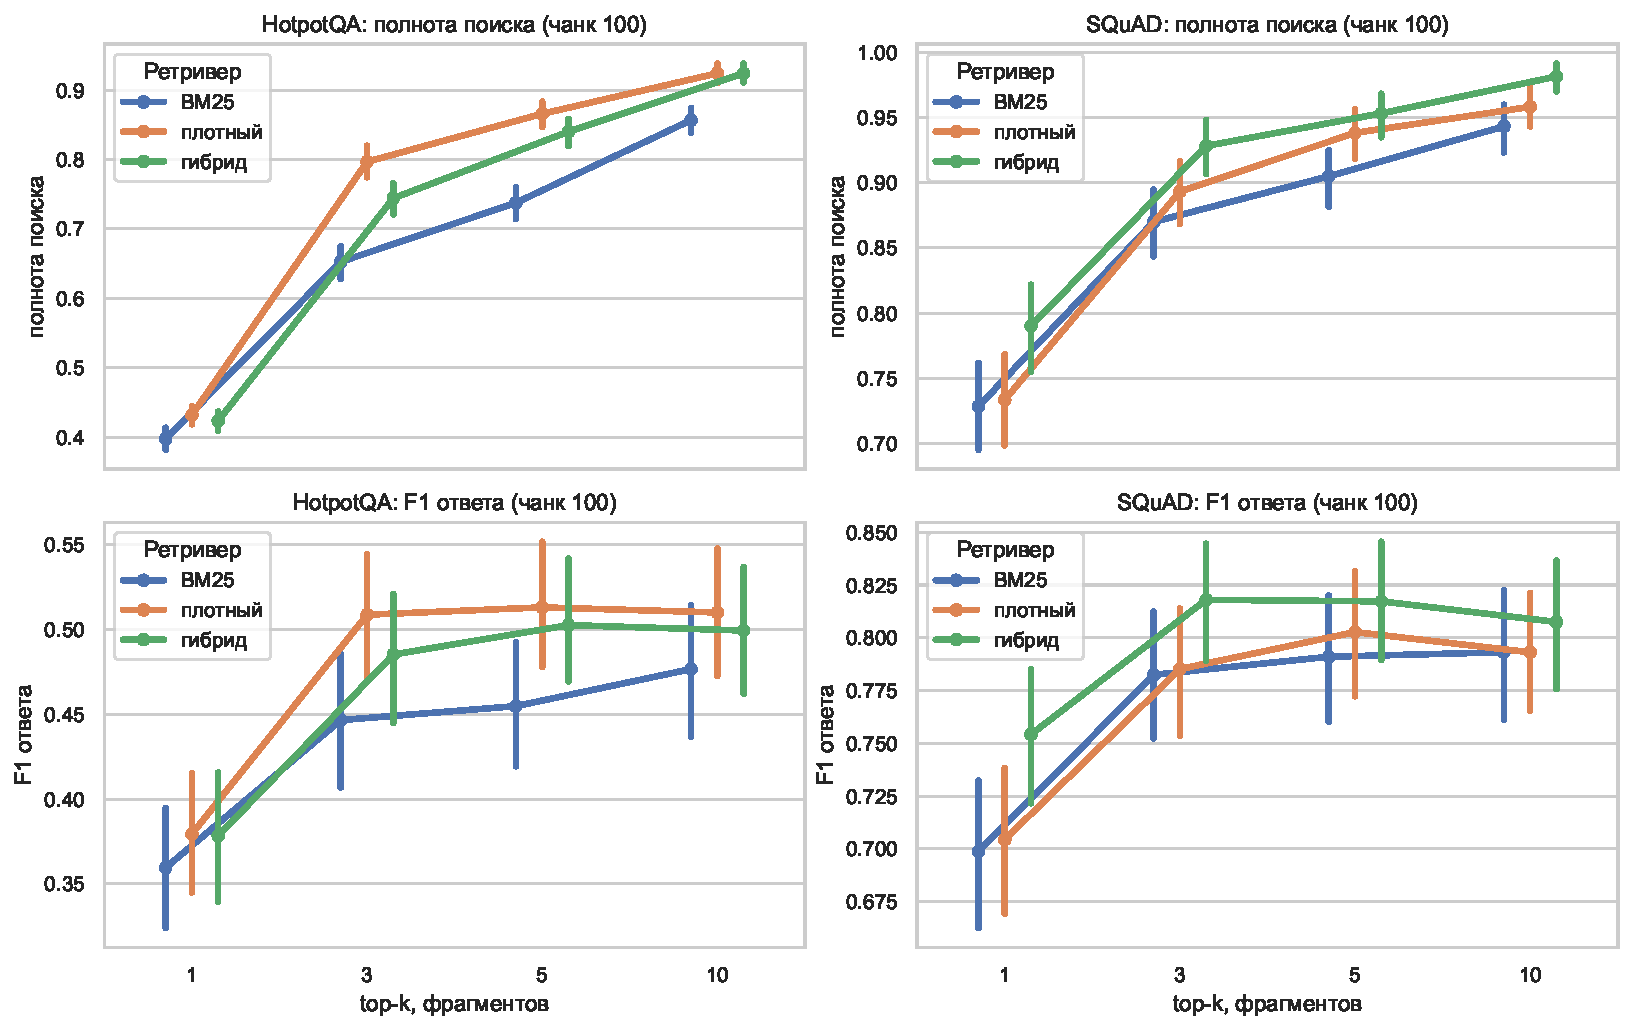
\includegraphics[width=0.92\linewidth]{figures/topk_curves.pdf}
\caption{Полнота поиска и F1 ответа в зависимости от top-k, чанк 100 слов, 95\,\% интервал}\label{fig:topk}
\end{figure}

\textbf{H3, размер чанка.} Крупные чанки повышают полноту: у HotpotQA 0,802, 0,840, 0,852 при 50, 100, 200 словах, у SQuAD 0,932, 0,953, 0,967. На F1 в парном тесте эффект не значим (HotpotQA 0,484, 0,503, 0,498). В регрессии по всей сетке эффект чанка значим, но мал: $\pm 0{,}01$ F1 (раздел~\ref{sec:reg}).

\textbf{H4, свойства вопроса.} Направление по типу вопроса обратно ожидаемому: comparison хуже bridge (F1 0,384 против 0,525, $n$ = 96 и 504, Манн--Уитни $p = 0{,}004$, рангово-бисериальная корреляция $-0{,}17$, знак минус означает перевес bridge). Тип вопроса распределен по уровням почти равномерно (comparison: 32, 29, 35 вопросов на easy, medium, hard), и с поправкой на уровень эффект сохраняется: $-0{,}142$ F1, $p = 0{,}005$ (МНК с ошибками HC3). Вопросы с ответом yes/no исключены из выборки; в train-части HotpotQA это 31\,\% comparison-вопросов (5\,481 из 17\,456), у bridge таких нет. Оставшиеся comparison-вопросы --- выбор одного из двух объектов, и вывод относится только к ним. Уровень сложности значим (Краскел--Уоллис $H = 33{,}6$, $p = 5{,}1 \cdot 10^{-8}$, $\varepsilon^2 = 0{,}056$; $\chi^2 = 26{,}7$ для доли правильных, V Крамера 0,21). Отличается только easy (F1 0,653) от medium (0,422) и hard (0,432), $p_{Holm} = 1{,}3 \cdot 10^{-6}$; medium и hard не различаются ($p = 0{,}92$).

\textbf{H5, ответ в контексте.} Если ответа в найденных чанках нет, правильных ответов почти нет: 3,3\,\% у HotpotQA и 13,0\,\% у SQuAD (последние --- частичные совпадения при F1~$\ge 0{,}5$). Если ответ в контексте есть, правильно отвечено 65,3\,\% и 85,8\,\% вопросов. Значит, у HotpotQA около трети ошибок при найденном ответе приходится на ридер, а не на поиск. На SQuAD релевантным считается чанк, содержащий ответ (раздел 4.3), поэтому там <<ответ в контексте>> почти совпадает с попаданием поиска, и для SQuAD H5 проверяет в основном ридер.

\textbf{H6, итерации} --- в разделе~\ref{sec:iter}.

\subsection{Корреляции параметров и метрик}

Корреляции Спирмена по всей сетке (21\,600 строк на датасет) показаны на рисунке~\ref{fig:corr}, ключевые пары --- в таблице~\ref{tab:corr}.

\begin{gosttable}{Корреляции Спирмена ключевых пар}\label{tab:corr}
\begin{tabular}{llrr}
\toprule
Параметр или свойство & Метрика & HotpotQA & SQuAD \\
\midrule
top-k & полнота поиска & 0,575 & 0,220 \\
top-k & F1 ответа & 0,087 & 0,061 \\
размер чанка & F1 ответа & 0,022 & 0,021 \\
слов в контексте & F1 ответа & 0,090 & 0,076 \\
длина вопроса & F1 ответа & 0,196 & 0,032 \\
лексическое пересечение & полнота поиска & 0,098 & 0,230 \\
лексическое пересечение & F1 ответа & 0,242 & 0,223 \\
оценка ретривера за первый чанк\footnotemark & полнота поиска & 0,099 & 0,265 \\
полнота поиска & F1 ответа & 0,328 & 0,566 \\
уверенность ридера & правильность & 0,369 & 0,475 \\
\bottomrule
\end{tabular}
\end{gosttable}
\footnotetext{Перцентиль оценки внутри ретривера и размера чанка: шкалы BM25, косинуса и RRF несравнимы.}

Все пары значимы после поправки Холма, но строки одного вопроса зависимы, поэтому $p$-значения здесь занижены и служат только описанием. Значимость проверена регрессией с кластерными ошибками. Параметры системы коррелируют с F1 слабо ($|\rho| < 0{,}1$), а свойства вопроса (пересечение, длина) и полнота поиска --- сильнее. Связь полноты и F1 на HotpotQA ($\rho = 0{,}33$) слабее, чем на SQuAD ($0{,}57$), но напрямую эти числа не сравнимы: на SQuAD релевантный чанк по определению содержит ответ, на HotpotQA --- опорное предложение. Внутри HotpotQA найденные нужные документы объясняют лишь часть качества ответа.

\begin{figure}[ht]
\centering
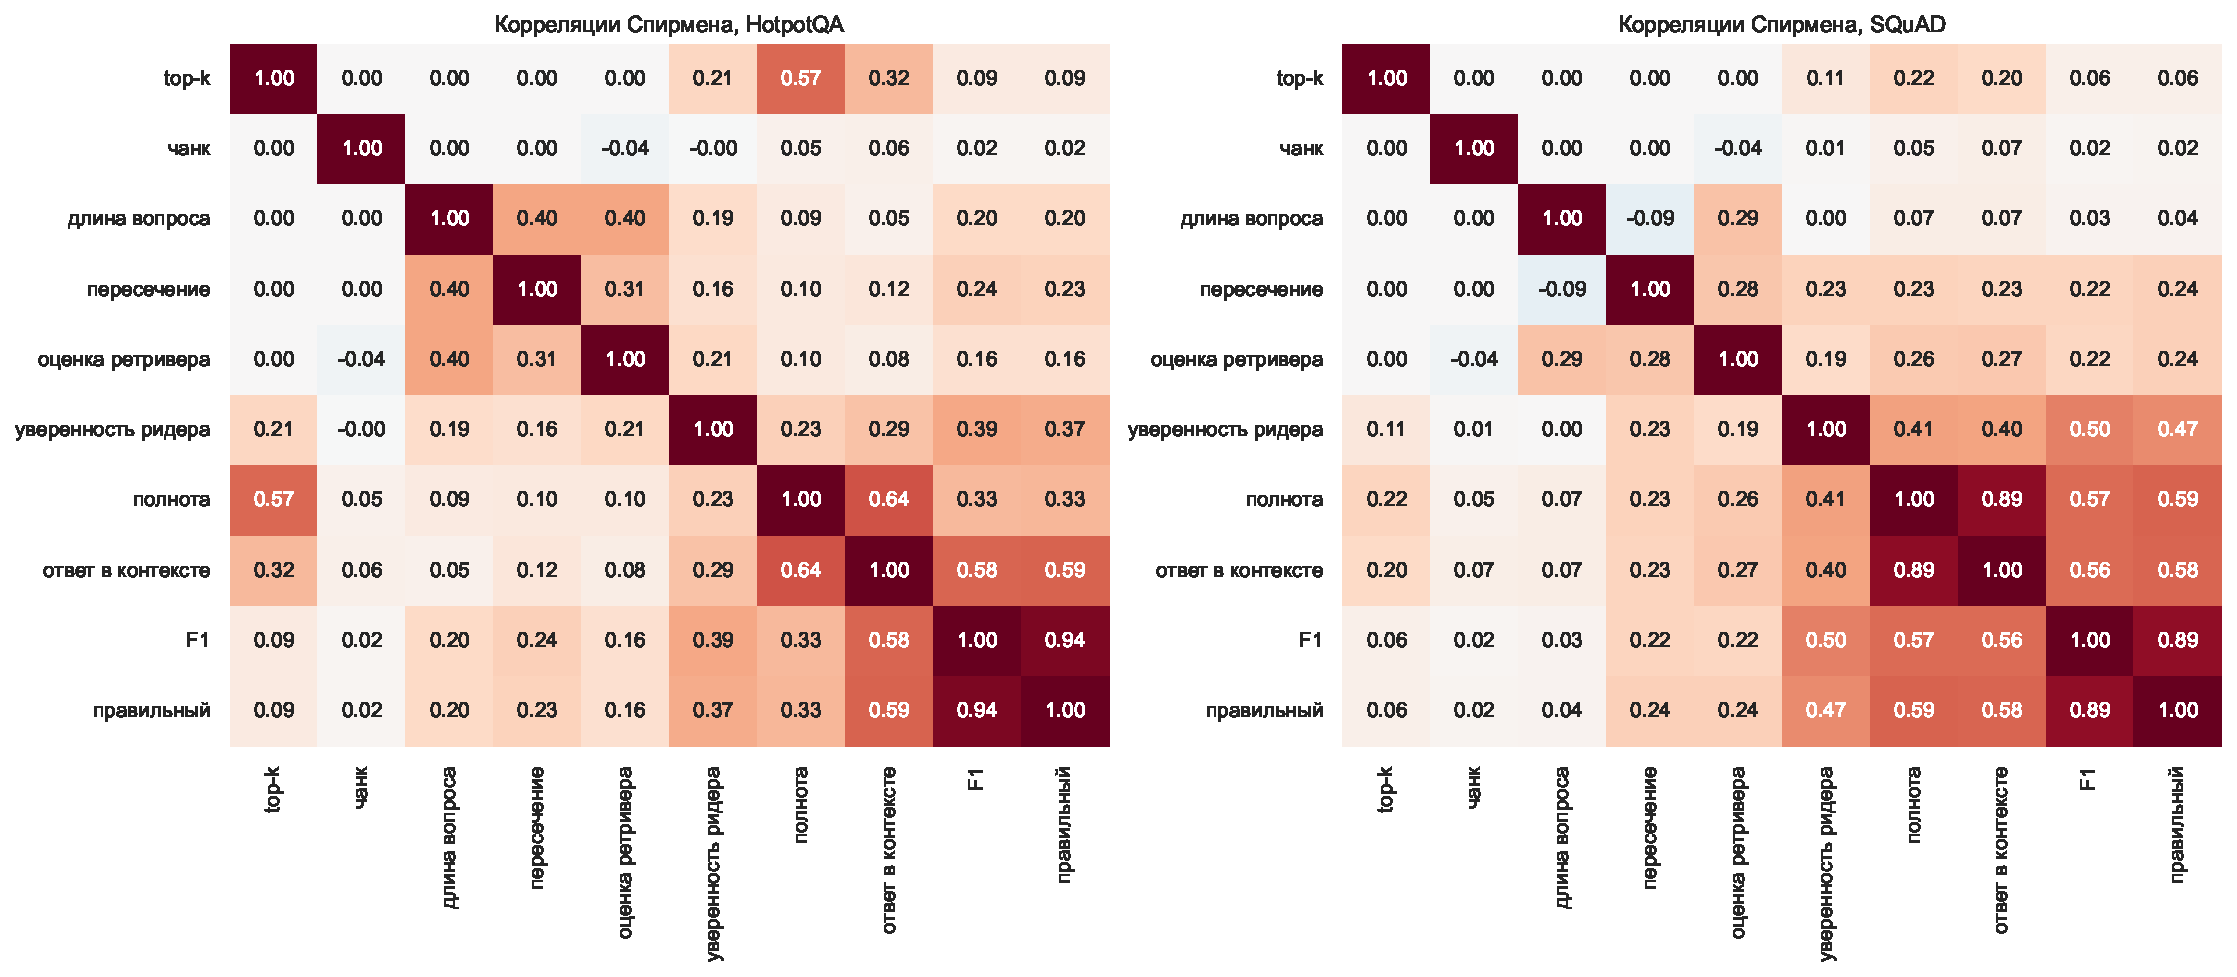
\includegraphics[width=\linewidth]{figures/spearman.pdf}
\caption{Матрицы корреляций Спирмена параметров и метрик}\label{fig:corr}
\end{figure}

\subsection{Регрессия качества по параметрам}\label{sec:reg}

Модель: F1 по ретриверу, датасету, $\log_2$ top-k, размеру чанка, длине вопроса, лексическому пересечению и числовому ответу; взаимодействия ретривера и top-k с датасетом. МНК, ошибки кластеризованы по вопросу (1\,200 кластеров, 43\,200 наблюдений). Коэффициенты --- в таблице~\ref{tab:ols}, база --- BM25, HotpotQA, чанк 100.

\begin{gosttable}{Регрессия F1 ответа, МНК с кластерными ошибками}\label{tab:ols}
\begin{tabular}{lrrr}
\toprule
Фактор & Коэффициент & 95\,\% интервал & $p$ \\
\midrule
Плотный ретривер & 0,043 & [0,027; 0,058] & $< 0{,}001$ \\
Гибридный ретривер & 0,030 & [0,021; 0,039] & $< 0{,}001$ \\
Плотный $\times$ SQuAD & $-0{,}034$ & [$-0{,}057$; $-0{,}011$] & 0,004 \\
Удвоение top-k ($\log_2 k$) & 0,037 & [0,029; 0,046] & $< 0{,}001$ \\
$\log_2 k$ $\times$ SQuAD & $-0{,}016$ & [$-0{,}026$; $-0{,}005$] & 0,004 \\
Чанк 50 слов & $-0{,}011$ & [$-0{,}022$; $-0{,}0004$] & 0,042 \\
Чанк 200 слов & 0,012 & [0,004; 0,019] & 0,002 \\
SQuAD & 0,507 & [0,462; 0,553] & $< 0{,}001$ \\
Длина вопроса, слово & 0,007 & [0,005; 0,009] & $< 0{,}001$ \\
Лексическое пересечение, 0 $\to$ 1 & 0,490 & [0,395; 0,586] & $< 0{,}001$ \\
Числовой ответ & $-0{,}062$ & [$-0{,}106$; $-0{,}019$] & 0,005 \\
\bottomrule
\end{tabular}
\end{gosttable}

$R^2 = 0{,}206$. Главное в разложении дисперсии: внутри одного датасета параметры системы (ретривер, top-k, чанк) объясняют 1,1\,\% дисперсии F1 на HotpotQA и 0,7\,\% на SQuAD, а фиксированный эффект вопроса --- 68\,\% и 60\,\%. Качество определяет прежде всего вопрос, параметры двигают среднее на единицы пунктов. Самый сильный фактор --- лексическое пересечение: рост на 0,1 добавляет 0,049 F1.

Логистическая модель правильности (GEE, обменная корреляция внутри вопроса) дает те же знаки: отношение шансов гибрида к BM25 1,20 [1,15; 1,25], плотного 1,15 [1,08; 1,23], на удвоение top-k 1,18 [1,14; 1,22], на чанк 200 против 100 --- 1,06 [1,02; 1,11]. Мультиколлинеарность низкая: VIF по матрице плана модели без взаимодействий не выше 1,43. Остатки МНК ненормальны из-за бимодальности F1 (приложение~\ref{app:diag}), поэтому выводы о значимости опираются на кластерные ошибки и GEE, а не на нормальную теорию.

\subsection{Классификация <<правильный/неправильный>>}

Задача --- предсказать правильность ответа (F1~$\ge 0{,}5$) по логу. Признаки берутся только из того, что система знает без эталона: параметры конфигурации, датасет, длина вопроса, число слов в контексте, перцентили оценок ретривера. Лексическое пересечение и числовой ответ сюда не входят: оба считаются по эталону. Три набора: <<до ридера без датасета>>, <<до ридера>> и <<с ридером>> (плюс уверенность ридера и ранг чанка с ответом). Проверка --- 5-кратная групповая кросс-валидация: все конфигурации одного вопроса в одном фолде.

\begin{gosttable}{Качество классификации правильности ответа, out-of-fold}\label{tab:clf}
\begin{tabular}{llrrrr}
\toprule
Модель & Признаки & ROC-AUC & PR-AUC & Accuracy & Брайер \\
\midrule
Всегда <<правильный>> & --- & 0,500 & 0,635 & 0,635 & 0,232 \\
Логит-регрессия & до ридера без датасета & 0,637 & 0,740 & 0,654 & 0,220 \\
Бустинг & до ридера без датасета & 0,711 & 0,794 & 0,681 & 0,205 \\
Логит-регрессия & до ридера & 0,737 & 0,808 & 0,695 & 0,195 \\
Бустинг & до ридера & 0,747 & 0,820 & 0,699 & 0,194 \\
Логит-регрессия & с ридером & 0,835 & 0,896 & 0,762 & 0,159 \\
Бустинг & с ридером & 0,837 & 0,886 & 0,766 & 0,159 \\
\bottomrule
\end{tabular}
\end{gosttable}

Результаты (таблица~\ref{tab:clf}, рисунок~\ref{fig:clf}): до ответа ридера правильность предсказуема с ROC-AUC 0,74--0,75, и большая часть этого --- знание датасета: без него 0,64 у логистической регрессии и 0,71 у бустинга. Уверенность ридера поднимает ROC-AUC до 0,84. По перестановочной важности главный признак --- уверенность ридера (падение ROC-AUC на 0,211), затем датасет (0,039), ранг чанка с ответом (0,028), длина вопроса (0,021) и перцентиль оценки ретривера (0,011); параметры конфигурации дают меньше 0,002 каждый. В логистической регрессии до ридера наибольший по модулю стандартизованный коэффициент --- у датасета ($-0{,}90$ для HotpotQA), затем перцентиль оценки ретривера (0,39) и длина вопроса (0,26).

\begin{figure}[ht]
\centering
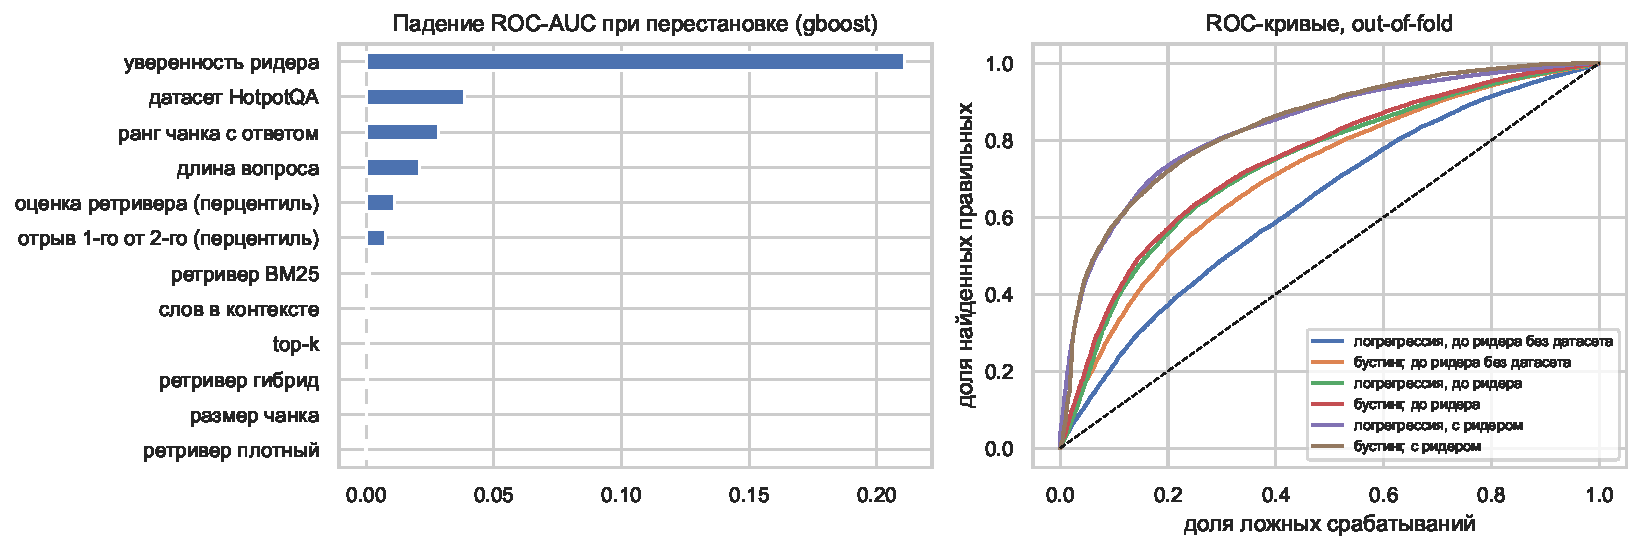
\includegraphics[width=0.95\linewidth]{figures/classification.pdf}
\caption{Перестановочная важность признаков и ROC-кривые}\label{fig:clf}
\end{figure}

\subsection{Динамика по итерациям поиска}\label{sec:iter}

\begin{gosttable}{Полнота и F1 по шагам итеративного поиска и при одношаговом поиске того же объема}\label{tab:iter}
\begin{tabular}{lrrrrrr}
\toprule
Датасет & Шаг & Чанков & \multicolumn{2}{c}{Полнота поиска} & \multicolumn{2}{c}{F1 ответа} \\
 & & & итеративный & одношаговый & итеративный & одношаговый \\
\midrule
\inputtab tables/tab_iterations.tex 
\bottomrule
\end{tabular}
\end{gosttable}

Средние по шагам --- в таблице~\ref{tab:iter}. Сравнение режимов на каждом шаге: Вилкоксон для F1 и полноты HotpotQA, Мак-Немар для бинарной полноты SQuAD, поправка Холма на три шага. На HotpotQA итеративный поиск находит нужные документы быстрее: на шаге 2 полнота 0,916 против 0,871 при одношаговом поиске того же объема (разность 0,045 [0,031; 0,059], $p_{Holm} = 1{,}7 \cdot 10^{-8}$), на шаге 3 --- 0,948 против 0,913 ($p_{Holm} = 2{,}2 \cdot 10^{-8}$), на шаге 4 --- 0,954 против 0,940 ($p_{Holm} = 0{,}011$). F1 по шагам на HotpotQA не меняется (Фридман $p = 0{,}17$, изменение с шага 1 на шаг 4 $+0{,}017$ [$-0{,}010$; $0{,}043$]).

На SQuAD итерации снижают полноту: на шаге 4 она 0,970 против 0,987 у одношагового поиска (Мак-Немар $p_{Holm} = 0{,}028$), на шаге 3 --- 0,963 против 0,978 ($p = 0{,}039$, после поправки $0{,}078$). F1 на SQuAD падает с ростом контекста в обоих режимах: в итеративном на 0,024 [0,007; 0,041] с шага 1 до шага 4 (Фридман $p = 0{,}0009$), в одношаговом на 0,015 [$-0{,}003$; 0,034]. На одном шаге режимы по F1 не различаются ($p_{Holm} \ge 0{,}70$), то есть итерации сами по себе F1 не снижают. Тест Пейджа односторонний и проверяет рост, поэтому падение видно по Фридману и бутстреп-интервалу.

GEE для правильности посчитан отдельно по датасетам, так как динамика в них разная. HotpotQA: отношение шансов на шаг 1,01 ($p = 0{,}51$), взаимодействие шага с режимом $p = 0{,}20$. SQuAD: 0,96 на шаг ($p = 0{,}067$), взаимодействие $p = 0{,}25$. Значимого влияния шага и различия режимов по правильности нет ни в одном наборе (рисунок~\ref{fig:iter}).

\begin{figure}[ht]
\centering
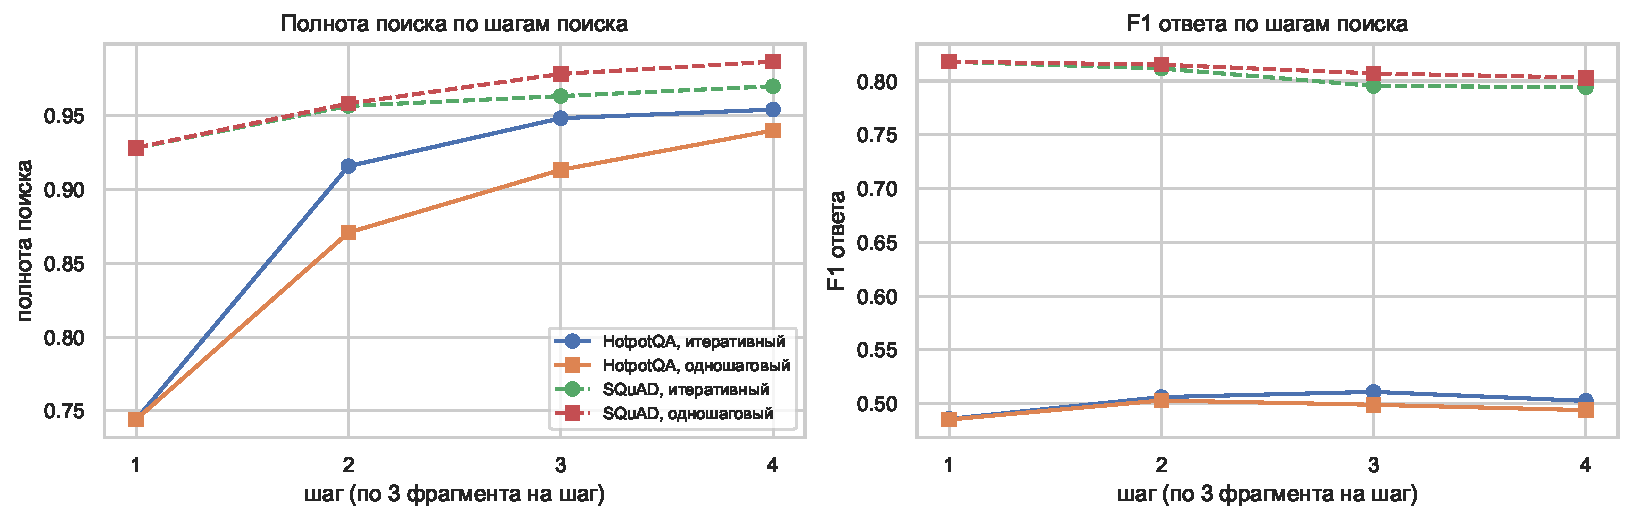
\includegraphics[width=\linewidth]{figures/iterations.pdf}
\caption{Полнота поиска и F1 ответа по шагам}\label{fig:iter}
\end{figure}

\section{Обсуждение и ограничения}

Параметры RAG значимо влияют на поиск: тип ретривера, top-k, размер чанка и итерации меняют полноту на 4--50 пунктов. На ответ они влияют на единицы пунктов, а прирост F1 после $k = 5$ не превышает 0,018. На одношаговых вопросах итерации снижают полноту, а F1 падает с ростом контекста в обоих режимах. Разброс качества определяется вопросом: его лексической близостью к документу, сложностью и типом. Отсюда практический вывод: сравнивать конфигурации RAG нужно парными тестами на одних вопросах. Межгрупповое сравнение средних тонет в разбросе между вопросами, который в 60--90 раз больше эффекта параметров.

На HotpotQA плотный поиск сильнее BM25, тогда как в BEIR~\cite{beir} BM25 часто сильнее плотных моделей вне домена обучения. Предобучение e5 включает пары текстов из Википедии, а дообучение --- MS MARCO и Natural Questions~\cite{e5}; пересечение этих данных с текстами HotpotQA и SQuAD не исключено, поэтому вывод о преимуществе e5 относится к корпусам этой работы.

\textbf{Ограничения.}
\begin{itemize}
\item Ридер экстрактивный (roberta-base-squad2), а не генеративная LLM. Выводы о потолке качества относятся к этому ридеру. Он обучен на SQuAD 2.0 train, куда входят вопросы SQuAD 1.1 train, поэтому на SQuAD он работает в своем домене и F1 там завышен относительно HotpotQA.
\item Корпус HotpotQA --- 5\,904 абзаца выбранных вопросов, а не вся Википедия. Абсолютная полнота выше, чем в открытой постановке; сравнения внутри сетки от этого не зависят.
\item Порог правильности F1~$\ge 0{,}5$ условный. Он засчитывает частичные совпадения, отсюда 13\,\% <<правильных>> ответов на SQuAD без ответа в контексте.
\item Корреляции и $p$-значения раздела 5.3 посчитаны по зависимым строкам и служат описанием.
\item Релевантность определена по-разному: на HotpotQA --- чанк с опорным предложением, на SQuAD --- чанк исходного абзаца с ответом. Полнота поиска на двух наборах поэтому не сравнима напрямую.
\item Вопросы HotpotQA взяты из train-части: dev-часть содержит только уровень hard. Ридер на HotpotQA не обучался.
\item Лексическое пересечение считается по эталонному документу. Это свойство вопроса для анализа, а не признак, доступный работающей системе; в классификацию оно не входит.
\item Comparison-вопросов 96, интервал для этой группы широкий.
\item Итерации --- шаги одного многошагового поиска, а не версии системы во времени. Глубина слияния RRF в итеративном и одношаговом режимах разная (60 и 50), отсюда расхождение F1 на шаге 1 в третьем знаке.
\item Плотная модель одна (e5-small-v2), размер выборки --- 600 вопросов на датасет, зерно одно.
\end{itemize}

\section{Выводы}

\begin{enumerate}
\item На HotpotQA и SQuAD прогнана система RAG по сетке из 72 конфигураций: 43\,200 строк лога ответов и 108\,000 строк лога поиска.
\item Тип ретривера значимо влияет на полноту поиска в обоих наборах и на F1: на HotpotQA плотный поиск лучше BM25 на 5,8 пункта, на SQuAD гибрид лучше BM25 на 2,6 пункта.
\item Полнота растет с top-k до $k = 10$, а прирост F1 от $k = 5$ к $k = 10$ не превышает 0,018 на HotpotQA и 0,004 на SQuAD (верхняя граница 95\,\% интервала).
\item Размер чанка влияет на полноту поиска, на F1 --- в пределах 0,01.
\item Внутри датасета параметры системы объясняют около 1\,\% дисперсии F1, вопрос --- 60--68\,\%. Сильнейший фактор --- лексическое пересечение вопроса и документа.
\item Правильность ответа предсказуема по логу без эталона с ROC-AUC 0,74--0,75 до ридера и 0,84 с его уверенностью.
\item Итеративный поиск повышает полноту на многошаговых вопросах на 4,5 пункта на шаге 2, а на одношаговых снижает ее к шагу 4 на 1,7 пункта. На F1 итерации сами по себе не влияют ни в одном наборе.
\end{enumerate}


\begin{thebibliography}{99}
\addcontentsline{toc}{section}{Список литературы}
\small
\bibitem{msmarco} Nguyen T., Rosenberg M., Song X. et al. MS MARCO: A Human Generated MAchine Reading COmprehension Dataset // CoCo Workshop at NIPS. --- 2016. --- arXiv:1611.09268.
\bibitem{nq} Kwiatkowski T., Palomaki J., Redfield O. et al. Natural Questions: A Benchmark for Question Answering Research // Transactions of the ACL. --- 2019. --- Vol.~7. --- P.~452--466.
\bibitem{hotpotqa} Yang Z., Qi P., Zhang S. et al. HotpotQA: A Dataset for Diverse, Explainable Multi-hop Question Answering // Proc. EMNLP. --- 2018. --- P.~2369--2380.
\bibitem{beir} Thakur N., Reimers N., Rücklé A. et al. BEIR: A Heterogeneous Benchmark for Zero-shot Evaluation of Information Retrieval Models // NeurIPS Datasets and Benchmarks Track. --- 2021.
\bibitem{squad} Rajpurkar P., Zhang J., Lopyrev K., Liang P. SQuAD: 100,000+ Questions for Machine Comprehension of Text // Proc. EMNLP. --- 2016. --- P.~2383--2392.
\bibitem{twowiki} Ho X., Duong Nguyen A.-K., Sugawara S., Aizawa A. Constructing A Multi-hop QA Dataset for Comprehensive Evaluation of Reasoning Steps // Proc. COLING. --- 2020.
\bibitem{musique} Trivedi H., Balasubramanian N., Khot T., Sabharwal A. MuSiQue: Multihop Questions via Single-hop Question Composition // Transactions of the ACL. --- 2022. --- Vol.~10.
\bibitem{triviaqa} Joshi M., Choi E., Weld D., Zettlemoyer L. TriviaQA: A Large Scale Distantly Supervised Challenge Dataset for Reading Comprehension // Proc. ACL. --- 2017. --- P.~1601--1611.
\bibitem{lewis2020} Lewis P., Perez E., Piktus A. et al. Retrieval-Augmented Generation for Knowledge-Intensive NLP Tasks // Advances in NeurIPS. --- 2020. --- Vol.~33. --- P.~9459--9474.
\bibitem{drqa} Chen D., Fisch A., Weston J., Bordes A. Reading Wikipedia to Answer Open-Domain Questions // Proc. ACL. --- 2017. --- P.~1870--1879.
\bibitem{gao2023} Gao Y., Xiong Y., Gao X. et al. Retrieval-Augmented Generation for Large Language Models: A Survey. --- 2023. --- arXiv:2312.10997.
\bibitem{bm25} Robertson S., Zaragoza H. The Probabilistic Relevance Framework: BM25 and Beyond // Foundations and Trends in Information Retrieval. --- 2009. --- Vol.~3, №~4. --- P.~333--389.
\bibitem{dpr} Karpukhin V., Oguz B., Min S. et al. Dense Passage Retrieval for Open-Domain Question Answering // Proc. EMNLP. --- 2020. --- P.~6769--6781.
\bibitem{e5} Wang L., Yang N., Huang X. et al. Text Embeddings by Weakly-Supervised Contrastive Pre-training. --- 2022. --- arXiv:2212.03533.
\bibitem{rrf} Cormack G.\,V., Clarke C.\,L.\,A., Büttcher S. Reciprocal Rank Fusion Outperforms Condorcet and Individual Rank Learning Methods // Proc. SIGIR. --- 2009. --- P.~758--759.
\bibitem{ragas} Es S., James J., Espinosa-Anke L., Schockaert S. RAGAS: Automated Evaluation of Retrieval Augmented Generation // Proc. EACL: System Demonstrations. --- 2024.
\bibitem{ares} Saad-Falcon J., Khattab O., Potts C., Zaharia M. ARES: An Automated Evaluation Framework for Retrieval-Augmented Generation Systems // Proc. NAACL. --- 2024.
\bibitem{erag} Salemi A., Zamani H. Evaluating Retrieval Quality in Retrieval-Augmented Generation // Proc. SIGIR. --- 2024.
\bibitem{lostmiddle} Liu N.\,F., Lin K., Hewitt J. et al. Lost in the Middle: How Language Models Use Long Contexts // Transactions of the ACL. --- 2024. --- Vol.~12. --- P.~157--173.
\bibitem{powernoise} Cuconasu F., Trappolini G., Siciliano F. et al. The Power of Noise: Redefining Retrieval for RAG Systems // Proc. SIGIR. --- 2024.
\bibitem{ircot} Trivedi H., Balasubramanian N., Khot T., Sabharwal A. Interleaving Retrieval with Chain-of-Thought Reasoning for Knowledge-Intensive Multi-Step Questions // Proc. ACL. --- 2023.
\bibitem{smucker2007} Smucker M.\,D., Allan J., Carterette B. A Comparison of Statistical Significance Tests for Information Retrieval Evaluation // Proc. CIKM. --- 2007. --- P.~623--632.
\bibitem{dror2018} Dror R., Baumer G., Shlomov S., Reichart R. The Hitchhiker's Guide to Testing Statistical Significance in Natural Language Processing // Proc. ACL. --- 2018. --- P.~1383--1392.
\bibitem{friedman} Friedman M. The Use of Ranks to Avoid the Assumption of Normality Implicit in the Analysis of Variance // JASA. --- 1937. --- Vol.~32, №~200. --- P.~675--701.
\bibitem{page} Page E.\,B. Ordered Hypotheses for Multiple Treatments: A Significance Test for Linear Ranks // JASA. --- 1963. --- Vol.~58, №~301. --- P.~216--230.
\bibitem{cochran} Cochran W.\,G. The Comparison of Percentages in Matched Samples // Biometrika. --- 1950. --- Vol.~37, №~3/4. --- P.~256--266.
\bibitem{mcnemar} McNemar Q. Note on the Sampling Error of the Difference Between Correlated Proportions or Percentages // Psychometrika. --- 1947. --- Vol.~12, №~2. --- P.~153--157.
\bibitem{holm} Holm S. A Simple Sequentially Rejective Multiple Test Procedure // Scandinavian Journal of Statistics. --- 1979. --- Vol.~6, №~2. --- P.~65--70.
\bibitem{efron} Efron B., Tibshirani R.\,J. An Introduction to the Bootstrap. --- New York: Chapman \& Hall, 1993. --- 436~p.
\bibitem{gee} Liang K.-Y., Zeger S.\,L. Longitudinal Data Analysis Using Generalized Linear Models // Biometrika. --- 1986. --- Vol.~73, №~1. --- P.~13--22.
\end{thebibliography}


\appendix
\renewcommand{\thesection}{\Asbuk{section}}
\section{Структура логов}\label{app:logs}
\begingroup\raggedright

\textbf{Лог ответов} (\texttt{answer\_log.parquet}, 43\,200 строк) --- строка на вопрос $\times$ конфигурацию: \texttt{dataset, qid, retriever, chunk\_size, top\_k}; свойства вопроса \texttt{q\_type, level, q\_len, answer\_len, answer\_is\_numeric, lex\_overlap}; поиск \texttt{hit\_at\_k, recall\_at\_k, mrr\_at\_k, answer\_in\_context, top1\_score, score\_margin, context\_words}; ответ \texttt{prediction, gold, reader\_score, pred\_rank, em, f1, correct}.

\textbf{Лог поиска} (\texttt{search\_log.parquet}, 108\,000 строк) --- строка на вопрос $\times$ ретривер $\times$ чанк $\times$ позицию выдачи 1--10: \texttt{chunk\_id, doc\_id, retrieval\_score, is\_relevant, has\_answer, reader\_answer, reader\_score}.

\textbf{Лог итераций} (\texttt{iteration\_log.parquet}, 9\,600 строк) --- строка на вопрос $\times$ режим $\times$ шаг: \texttt{query\_len, context\_words, recall, hit, answer\_in\_context, prediction, em, f1, correct}.

\par\endgroup

\section{Метрики по всей сетке}\label{app:grid}

\begin{gosttable}{F1 ответа по конфигурациям, HotpotQA}
\begin{tabular}{lrrrrr}
\toprule
Ретривер & Чанк, слов & top-1 & top-3 & top-5 & top-10 \\
\midrule
\inputtab tables/tab_grid_hotpot_f1.tex 
\bottomrule
\end{tabular}
\end{gosttable}

\begin{gosttable}{F1 ответа по конфигурациям, SQuAD}
\begin{tabular}{lrrrrr}
\toprule
Ретривер & Чанк, слов & top-1 & top-3 & top-5 & top-10 \\
\midrule
\inputtab tables/tab_grid_squad_f1.tex 
\bottomrule
\end{tabular}
\end{gosttable}

\begin{gosttable}{Полнота поиска по конфигурациям, HotpotQA}
\begin{tabular}{lrrrrr}
\toprule
Ретривер & Чанк, слов & top-1 & top-3 & top-5 & top-10 \\
\midrule
\inputtab tables/tab_grid_hotpot_recall.tex 
\bottomrule
\end{tabular}
\end{gosttable}

\begin{gosttable}{Полнота поиска по конфигурациям, SQuAD}
\begin{tabular}{lrrrrr}
\toprule
Ретривер & Чанк, слов & top-1 & top-3 & top-5 & top-10 \\
\midrule
\inputtab tables/tab_grid_squad_recall.tex 
\bottomrule
\end{tabular}
\end{gosttable}

\section{Диагностика регрессии}\label{app:diag}

\begin{figure}[H]
\centering
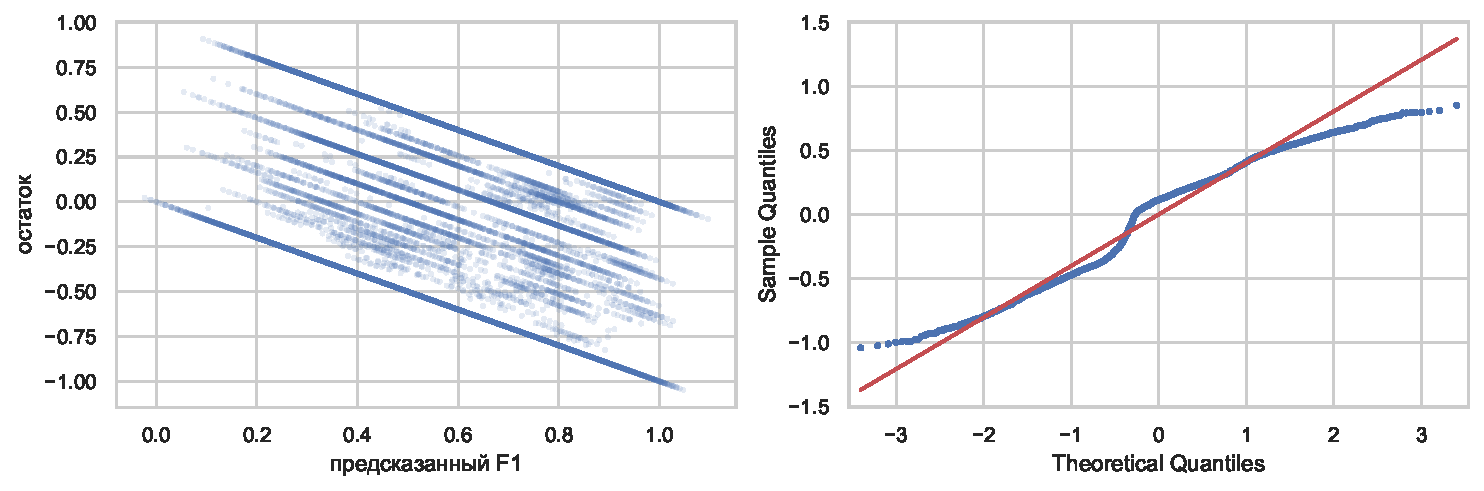
\includegraphics[width=0.9\linewidth]{figures/ols_diagnostics.pdf}
\caption{Остатки МНК против предсказания и Q-Q график остатков}
\end{figure}

\section{Воспроизведение}\label{app:repro}

Код --- репозиторий \texttt{stat-rag}, Python 3.11, менеджер окружения uv. Зерно выборки 42. Прогон сетки на Apple M4 Pro --- 13 минут, итеративный прогон --- 3,5 минуты, анализ --- около минуты. Скачивается около 350~МБ (HotpotQA train --- 326~МБ). Ревизии моделей и датасетов на Hugging Face закреплены в коде. Логи прогона лежат в репозитории, поэтому анализ и отчет пересобираются без повторного прогона за пару минут. Сборка PDF --- xelatex трижды, нужны шрифты PT Serif, PT Sans, PT Mono.

\begin{Verbatim}[fontsize=\small]
uv sync
uv run python scripts/download_data.py
uv run python src/stat_rag/run_grid.py
uv run python src/stat_rag/run_iterative.py
uv run python notebooks/build_notebook.py
uv run jupyter nbconvert --to notebook --execute --inplace notebooks/analysis.ipynb
uv run python report/make_tables.py
cd report && xelatex <отчет>.tex  # трижды
uv run pytest tests/ -q
\end{Verbatim}

\end{document}
